For reference, we tabulate the mean revenue underlying the acceptance-rate
results of Section~\ref{sec:acceptance}. Revenue tracks acceptance but smooths
over the bimodal collapse of the disjoint baseline, which is why we report
acceptance as the primary metric. Each value is the average of 15 CPLEX runs
under a time and optimality-gap limit.

\begin{table}[H]
\caption{Revenue of joint vs. disjoint on FatTree (\(k = 6\), default VNFM).}
\label{tbl:fattree}
\begin{tabularx}{0.7\textwidth}{Xrr}
\toprule
\textbf{Chains} & \textbf{Joint} & \textbf{Disjoint} \\
\midrule
10 & 4453 & 1913 \\
15 & 6587 & 1000 \\
20 & 8887 & 1593 \\
25 & 11{,}133 & 3267 \\
30 & 13{,}327 & 7907 \\
35 & 15{,}467 & 13{,}073 \\
40 & 17{,}973 & 14{,}687 \\
45 & 20{,}147 & 17{,}553 \\
50 & 22{,}440 & 15{,}633 \\
55 & 24{,}447 & 14{,}613 \\
60 & 26{,}940 & 14{,}713 \\
65 & 29{,}313 & 18{,}887 \\
70 & 31{,}487 & 16{,}313 \\
75 & 33{,}713 & 17{,}340 \\
80 & 36{,}253 & 19{,}553 \\
85 & 37{,}847 & 18{,}540 \\
90 & 40{,}500 & 23{,}360 \\
\bottomrule
\end{tabularx}
\end{table}

\begin{figure}[H]
\centering
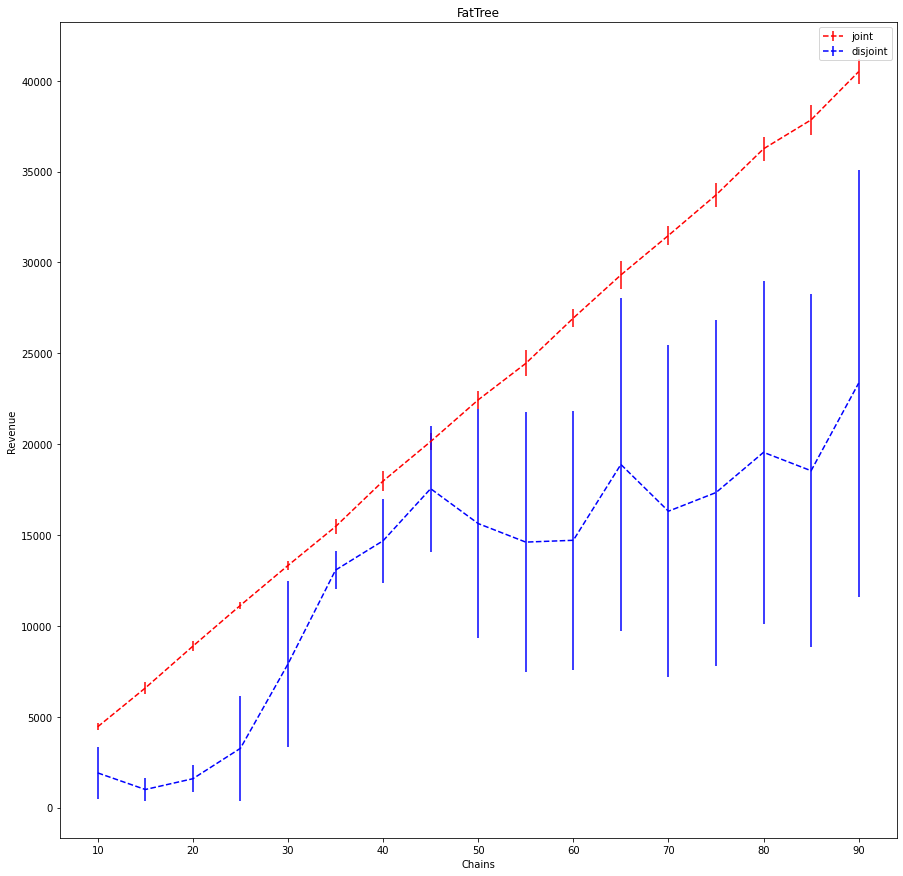
\includegraphics[width=0.7\textwidth]{plots/joint-vs-disjoint-fattree.png}
\caption{Revenue of joint vs. disjoint on FatTree (\(k = 6\)).}
\label{fig:fattree}
\end{figure}

With the \emph{default} (slack) management settings the joint and disjoint
solutions earn essentially identical revenue on USNet
(Table~\ref{tbl:usnet-slack}, Figure~\ref{fig:usnet-slack}): the topology can
manage every chain, so the management constraint does not bind.

\begin{table}[H]
\caption{Revenue of joint vs. disjoint on USNet (slack management).}
\label{tbl:usnet-slack}
\begin{tabularx}{0.7\textwidth}{Xrr}
\toprule
\textbf{Chains} & \textbf{Joint} & \textbf{Disjoint} \\
\midrule
50 & 23{,}000 & 23{,}010 \\
75 & 34{,}180 & 34{,}260 \\
100 & 45{,}430 & 45{,}560 \\
125 & 57{,}180 & 57{,}380 \\
150 & 68{,}750 & 69{,}360 \\
\bottomrule
\end{tabularx}
\end{table}

\begin{figure}[H]
\centering
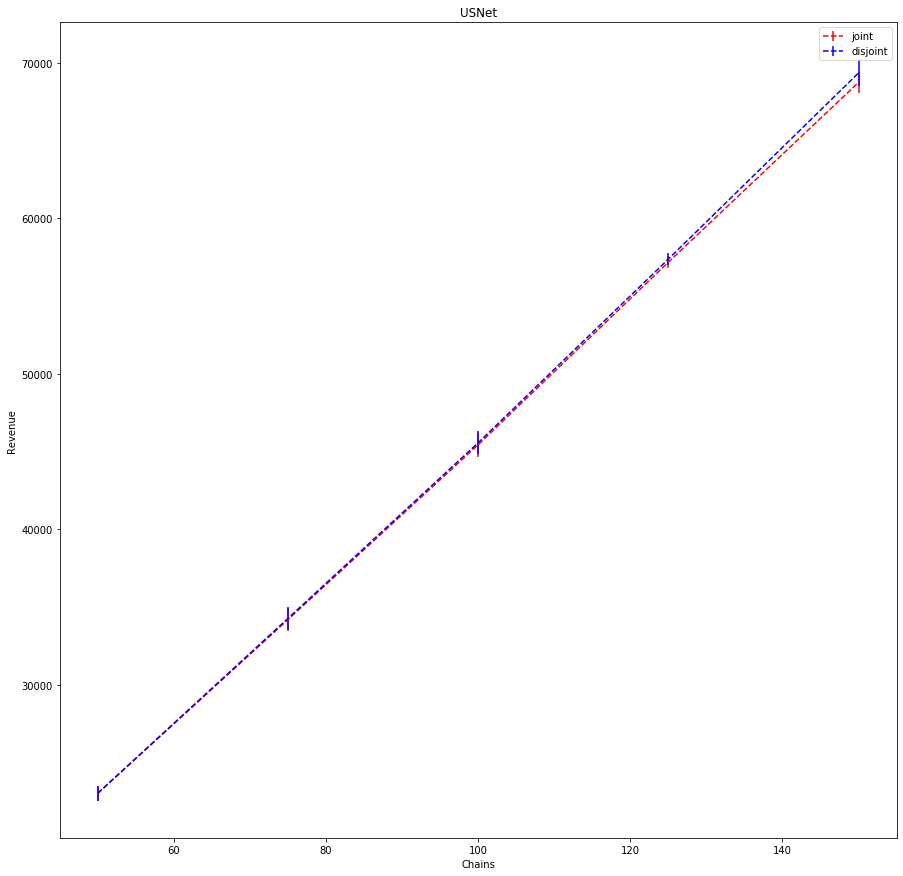
\includegraphics[width=0.7\textwidth]{plots/joint-vs-disjoint-usnet-1.png}
\caption{Revenue of joint vs. disjoint on USNet (slack management).}
\label{fig:usnet-slack}
\end{figure}

When the manager radius is tightened to 4 hops the constraint binds and the joint
advantage reappears in revenue as well (Table~\ref{tbl:usnet-tight},
Figure~\ref{fig:usnet-tight}).

\begin{table}[H]
\caption{Revenue of joint vs. disjoint on USNet (4-hop management radius).}
\label{tbl:usnet-tight}
\begin{tabularx}{0.7\textwidth}{Xrr}
\toprule
\textbf{Chains} & \textbf{Joint} & \textbf{Disjoint} \\
\midrule
10 & 4473 & 1420 \\
15 & 6927 & 2733 \\
20 & 8940 & 3533 \\
25 & 11{,}133 & 4833 \\
30 & 13{,}313 & 9020 \\
35 & 15{,}487 & 14{,}693 \\
40 & 17{,}913 & 15{,}433 \\
45 & 19{,}813 & 17{,}587 \\
50 & 22{,}213 & 21{,}020 \\
55 & 24{,}113 & 21{,}867 \\
60 & 26{,}640 & 24{,}547 \\
65 & 28{,}833 & 25{,}760 \\
70 & 31{,}360 & 29{,}420 \\
75 & 33{,}140 & 29{,}660 \\
80 & 35{,}687 & 33{,}320 \\
85 & 37{,}600 & 34{,}987 \\
90 & 39{,}840 & 37{,}473 \\
\bottomrule
\end{tabularx}
\end{table}

\begin{figure}[H]
\centering
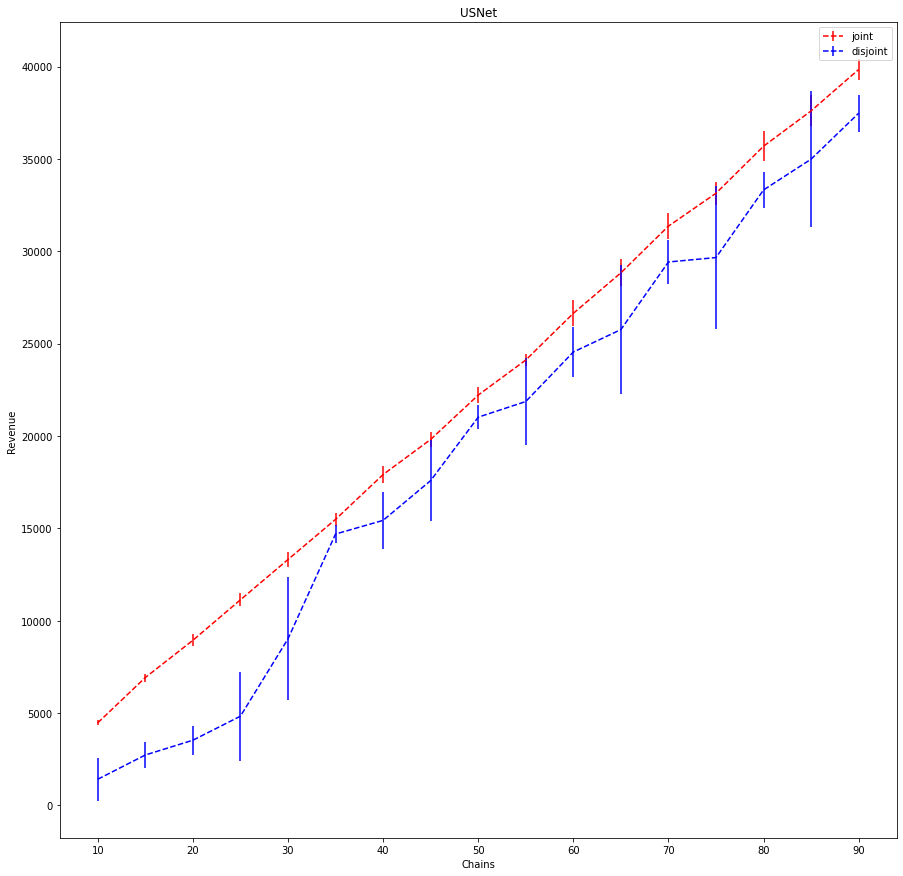
\includegraphics[width=0.7\textwidth]{plots/joint-vs-disjoint-usnet-2.png}
\caption{Revenue of joint vs. disjoint on USNet (4-hop management radius).}
\label{fig:usnet-tight}
\end{figure}
